\documentclass[12pt]{article}
\usepackage{sbc-template}
\usepackage[utf8]{inputenc}
\usepackage[brazilian]{babel}
% Compatibilidade babel >= 2024 x sbc-template.sty (2001): o template
% redefine \normalsize (linha 31 do .sty), o que quebra a maquinaria de
% \normalsfcodes que o babel moderno espera no gancho begindocument/before,
% causando "Undefined control sequence" (\bbl@normalsf) em \begin{document}.
% Definimos os dois comandos como no-op para restaurar a compatibilidade.
\makeatletter
\providecommand{\normalsfcodes}{}
\providecommand{\bbl@normalsf}{}
\makeatother
\usepackage{graphicx,url}
\usepackage{booktabs}
\usepackage{amsmath}
\usepackage{hyperref}
\sloppy

% Macros e figuras gerados por analise.py
\newcommand{\nTotal}{11.055}
\newcommand{\nFeatures}{30}
\newcommand{\nPhishing}{6.157}
\newcommand{\nLegitimo}{4.898}
\newcommand{\pctPhishing}{55{,}7\%}
\newcommand{\friedmanChi}{56{,}27}
\newcommand{\friedmanP}{< 0{,}001}
\newcommand{\melhorModelo}{Random Forest}
\newcommand{\melhorFOne}{0{,}974}
\newcommand{\melhorAUC}{0{,}998}
\newcommand{\melhorAcuracia}{0{,}974}
\newcommand{\melhorSigmaCV}{0{,}004}
\newcommand{\naiveBayesFOne}{0{,}561}
\newcommand{\pcaVarUm}{15{,}5\%}
\newcommand{\pcaVarDois}{11{,}8\%}
\newcommand{\topDoisPct}{56{,}7\%}

\graphicspath{{resultados/figuras/}}

\title{Detecção de Phishing em URLs com Classificadores Clássicos:\\
       Um Estudo Comparativo}

\author{Vinícius Magalhães Dias\inst{1}, João Marcello Machado Braz\inst{1},
        Pedro Gabryel Araujo do Nascimento\inst{1}}

\address{Disciplina de Reconhecimento de Padrões\\
  [PREENCHER: Instituição] -- [Cidade], [UF] -- Brasil
  \email{[PREENCHER: emails separados por vírgula]}}

\begin{document}
\maketitle

\begin{abstract}
This paper evaluates seven classical classifiers on the task of phishing URL
detection using the UCI Phishing Websites dataset (\nTotal{} samples,
\nFeatures{} categorical attributes). Models were assessed through stratified
10-fold cross-validation and on a held-out test set, using accuracy, macro
F1-score, and AUC-ROC as metrics. \melhorModelo{} achieved the best results
($\text{F1} = \melhorFOne{}$, $\text{AUC-ROC} = \melhorAUC{}$).
A Friedman statistical test confirmed that performance differences across
classifiers are significant ($\chi^{2} = \friedmanChi{}$,
$p \friedmanP{}$). Feature importance analysis indicates that SSL certificate
status and the proportion of external anchor URLs are the most
discriminative attributes.
\end{abstract}

\begin{resumo}
Este trabalho avalia sete classificadores clássicos na tarefa de detecção de
URLs de phishing usando o dataset UCI Phishing Websites (\nTotal{} amostras,
\nFeatures{} atributos categóricos). Os modelos foram avaliados por validação
cruzada estratificada de 10 folds e em conjunto de teste separado, com métricas
de acurácia, F1 macro e AUC-ROC. \melhorModelo{} obteve o melhor desempenho
($\text{F1} = \melhorFOne{}$, $\text{AUC-ROC} = \melhorAUC{}$).
O teste de Friedman confirmou diferenças estatisticamente significativas entre
os classificadores ($\chi^{2} = \friedmanChi{}$, $p \friedmanP{}$). A análise
de importância indica que o estado do certificado SSL e a proporção de âncoras
externas são os atributos mais discriminativos do conjunto de dados.
\end{resumo}

\section{Introdução}

Phishing é uma técnica de engenharia social na qual o atacante cria URLs
fraudulentas que imitam serviços legítimos para roubar credenciais ou induzir
a instalação de malware~\cite{verma2017}. O volume do problema é expressivo:
somente em 2023, a Anti-Phishing Working Group registrou cerca de cinco milhões
de ataques de phishing, o maior total anual de sua série histórica~\cite{apwg2023}.
Nesse cenário, a triagem puramente manual é inviável; filtros
automáticos baseados em aprendizado de máquina tornaram-se componentes
essenciais de browsers, gateways de e-mail e proxies corporativos. A
efetividade desses sistemas depende da escolha adequada do classificador e
dos atributos extraídos da URL.

Este trabalho compara sete classificadores clássicos de aprendizado de
máquina — Regressão Logística, Naive Bayes Gaussiano, KNN, Árvore de
Decisão, Random Forest, SVM com kernel RBF e Gradient Boosting — na tarefa
de detecção de phishing em URLs usando o dataset UCI Phishing
Websites~\cite{mohammad2012}, com \nTotal{} amostras e \nFeatures{} atributos
categóricos. A avaliação combina validação cruzada de 10 folds com teste
estatístico de Friedman para verificar a significância das diferenças de
desempenho.

\section{Trabalhos Relacionados}

Mohammad et al.~\cite{mohammad2012} propuseram o dataset UCI Phishing Websites
e um sistema de classificação baseado em regras derivadas dos \nFeatures{}
atributos extraídos manualmente de URL, DNS e HTML, reportando acurácia de
92,4\% com classificação fuzzy. O dataset tornou-se referência amplamente
adotada em pesquisas subsequentes sobre o tema.

Sahingoz et al.~\cite{sahingoz2019} compararam sete algoritmos de aprendizado
de máquina em um conjunto de URLs coletadas em tempo real, usando atributos
léxicos e de conteúdo. Random Forest obteve acurácia de 97,98\% e foi o
melhor modelo no estudo, na mesma faixa da acurácia de \melhorAcuracia{}
alcançada pelo Random Forest neste trabalho.

Jain e Gupta~\cite{jain2018} propuseram um classificador baseado em
hiperlinks extraídos do lado do cliente, sem acesso ao conteúdo da página,
alcançando acurácia de 98,4\%. A abordagem é relevante por dispensar o
carregamento da página, reduzindo latência na detecção.

Verma e Das~\cite{verma2017} investigaram extração rápida de atributos
léxicos da string da URL para detecção de URLs maliciosas, mostrando que
características simples como comprimento, uso de subdomínios e presença de
caracteres especiais são altamente discriminativas, mesmo sem análise do
conteúdo da página.

\section{Fundamentação Teórica}

Os sete classificadores avaliados diferem em hipóteses de indução e
complexidade computacional. Regressão Logística estima a probabilidade
posterior de cada classe como função sigmoidal de uma combinação linear dos
atributos padronizados, sendo eficiente e interpretável. Naive Bayes Gaussiano
assume independência condicional entre atributos e distribuição normal dentro
de cada classe; a violação dessas hipóteses em dados categóricos pode degradar
significativamente o desempenho~\cite{demsar2006}. $K$-Nearest Neighbors
($k=5$)~\cite{cover1967} classifica por maioria de votos dos $k$ vizinhos mais
próximos no espaço padronizado, sem fase de treino explícita, mas com custo de
predição linear no tamanho do conjunto de treino. Árvore de Decisão particiona
recursivamente o espaço de atributos maximizando a redução de impureza de
Gini~\cite{breiman1984}, produzindo regras diretamente interpretáveis. Random Forest constrói
um ensemble de árvores sobre subconjuntos aleatórios dos dados e dos atributos,
reduzindo variância por agregação e fornecendo estimativas naturais de
importância de atributos~\cite{breiman2001}. Máquina de Vetores de Suporte
com kernel RBF mapeia os dados para um espaço de maior dimensão e encontra
o hiperplano de margem máxima nesse espaço~\cite{cortes1995}; a padronização
dos atributos é essencial para o funcionamento correto do kernel. Gradient
Boosting~\cite{friedman2001} treina uma sequência de árvores rasas de forma
aditiva, onde cada árvore corrige os resíduos da anterior, obtendo modelos de
alta acurácia ao custo de maior tempo de treino; implementações escaláveis
desse paradigma, como o XGBoost~\cite{chen2016}, difundiram seu uso em
aplicações de larga escala.

\section{Metodologia}

\subsection{Dataset}

O dataset UCI Phishing Websites~\cite{mohammad2012} contém \nTotal{} amostras
descritas por \nFeatures{} atributos categóricos de valor ternário
$\{-1, 0, 1\}$, extraídos de características da URL, do servidor DNS, do
código HTML e do comportamento JavaScript da página. São \nPhishing{} amostras
de phishing (\pctPhishing{}) e \nLegitimo{} legítimas, configurando um leve
desbalanceamento. Não há valores faltantes. Os rótulos seguem a convenção
$+1$ para phishing e $-1$ para legítimo.

\subsection{Configuração Experimental}

Os dados foram divididos em treino (80\%) e teste (20\%) com estratificação
por classe e \texttt{random\_state=42}, garantindo reprodutibilidade. Os
hiperparâmetros seguiram os valores padrão da literatura: \texttt{n\_estimators=200}
para Random Forest e Gradient Boosting, $k=5$ para KNN e \texttt{max\_iter=2000}
para a Regressão Logística. Classificadores sensíveis à escala — Regressão
Logística, Naive Bayes, KNN e SVM — receberam os atributos padronizados via
\texttt{StandardScaler} dentro de um \texttt{Pipeline}. Os demais operaram
sobre os dados brutos. Toda a implementação — modelos, padronização, validação
cruzada e métricas — utilizou a biblioteca scikit-learn~\cite{pedregosa2011}.

\subsection{Avaliação e Teste Estatístico}

A avaliação principal utilizou validação cruzada estratificada de 10 folds
no conjunto de treino, coletando acurácia, F1 macro e AUC-ROC por fold.
Os modelos foram então treinados em todo o conjunto de treino e avaliados
no conjunto de teste. Para determinar se as diferenças de desempenho são
estatisticamente significativas, aplicou-se o teste não paramétrico de
Friedman~\cite{demsar2006} sobre os escores de F1 macro por fold, seguido
pelo pós-teste de Nemenyi para comparações par a par.

\section{Resultados e Discussão}

A Tabela~\ref{tab:principal} apresenta os resultados completos em validação
cruzada e no conjunto de teste. \melhorModelo{} obteve o melhor desempenho
geral, com acurácia de \melhorAcuracia{}, $\text{F1} = \melhorFOne{}$ e
$\text{AUC-ROC} = \melhorAUC{}$ no
conjunto de teste, e variância reduzida na validação cruzada
($\sigma = \melhorSigmaCV{}$), indicando estabilidade. A Árvore de Decisão
acompanhou o Random Forest de perto em F1 (0{,}971), enquanto Gradient Boosting,
SVM RBF e KNN formaram um grupo intermediário (F1 entre 0{,}949 e 0{,}956) e a
Regressão Logística ficou logo abaixo (0{,}927). Naive Bayes registrou desempenho
significativamente inferior ao dos demais, com F1 de $\naiveBayesFOne{}$,
reflexo direto da violação da suposição gaussiana: os atributos do dataset
são categóricos ternários, incompatíveis com a hipótese de normalidade do
modelo.

\begin{table}[htb]
\centering
\caption{Desempenho dos classificadores em validação cruzada de 10 folds
(CV) e no conjunto de teste. F1 refere-se à média macro.}
\label{tab:principal}
\begin{tabular}{lcccc}
\hline
\textbf{Classificador} & \textbf{F1 (CV, $\mu\pm\sigma$)} & \textbf{F1 (teste)} & \textbf{AUC-ROC} & \textbf{Tempo (s)} \\
\hline
    Regressão Logística & 0{,}926 $\pm$ 0{,}006 & 0{,}927 & 0{,}981 & 0{,}01 \\
    Naive Bayes & 0{,}561 $\pm$ 0{,}012 & 0{,}561 & 0{,}970 & 0{,}00 \\
    KNN (k=5) & 0{,}940 $\pm$ 0{,}005 & 0{,}949 & 0{,}987 & 0{,}00 \\
    Árvore de Decisão & 0{,}961 $\pm$ 0{,}006 & 0{,}971 & 0{,}980 & 0{,}01 \\
    Random Forest & 0{,}970 $\pm$ 0{,}004 & 0{,}974 & 0{,}998 & 0{,}17 \\
    SVM RBF & 0{,}948 $\pm$ 0{,}006 & 0{,}951 & 0{,}989 & 2{,}14 \\
    Gradient Boosting & 0{,}952 $\pm$ 0{,}005 & 0{,}956 & 0{,}994 & 0{,}75 \\
\hline
\end{tabular}

\end{table}

As curvas ROC (Figura~\ref{fig:roc}) complementam a análise por F1. Os
modelos de ensemble alcançam AUC-ROC próximo do ótimo (Random Forest 0{,}998
e Gradient Boosting 0{,}994), indicando forte discriminação em todos os
limiares. A Árvore de Decisão, apesar do segundo melhor F1, apresenta o AUC-ROC
mais baixo entre os modelos não triviais (0{,}980): por produzir probabilidades
pouco graduadas, ela decide bem no limiar padrão, mas discrimina de forma menos
consistente ao longo de todos os limiares. A curva de Naive Bayes, apesar de
AUC-ROC competitivo, colapsa
em F1 muito inferior porque a distribuição de probabilidades geradas pelo
modelo é mal calibrada: as suposições de independência do Naive Bayes empurram
as probabilidades estimadas para os extremos 0 e 1~\cite{niculescu2005},
tornando o limiar padrão de 0,5 inadequado.

\begin{figure}[htb]
\centering
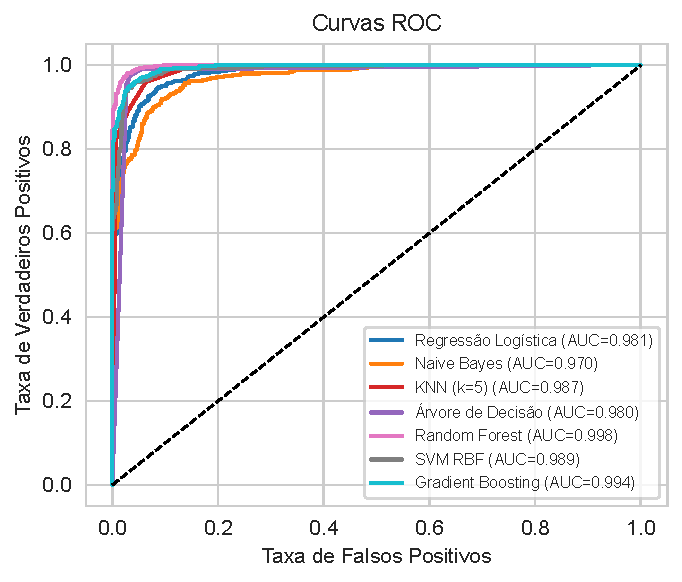
\includegraphics[width=\columnwidth]{curvas_roc.pdf}
\caption{Curvas ROC dos sete classificadores avaliados no conjunto de teste.}
\label{fig:roc}
\end{figure}

O teste de Friedman resultou em $\chi^{2} = \friedmanChi{}$
($p \friedmanP{}$), rejeitando a hipótese nula de desempenho estatisticamente
equivalente entre todos os classificadores. O pós-teste de Nemenyi revelou
que Naive Bayes difere significativamente de todos os demais modelos
($p < 0{,}05$), ao passo que as diferenças entre os outros seis classificadores
não atingem significância estatística nesse critério, sugerindo que todos
são escolhas viáveis para o problema. Do ponto de vista de custo, o tempo de
treino também favorece o Random Forest: ele foi treinado em fração de segundo,
enquanto o SVM RBF foi o mais custoso (cerca de 2~s, uma ordem de grandeza
acima dos demais), sem oferecer ganho de desempenho que justifique o custo
adicional.

A Figura~\ref{fig:importancia} mostra os quinze atributos de maior importância
segundo o \melhorModelo{}. Os dois mais relevantes — \texttt{sslfinal\_state}
(estado do certificado SSL) e \texttt{url\_of\_anchor} (proporção de âncoras
externas) — respondem juntos por \topDoisPct{} da importância total, indicando
que indicadores de segurança do protocolo e de comportamento de hiperlinks da
página concentram a maior parte do poder discriminativo. Os atributos restantes
contribuem de forma mais distribuída, sem nenhum outro com importância
individual relevante.

\begin{figure}[htb]
\centering
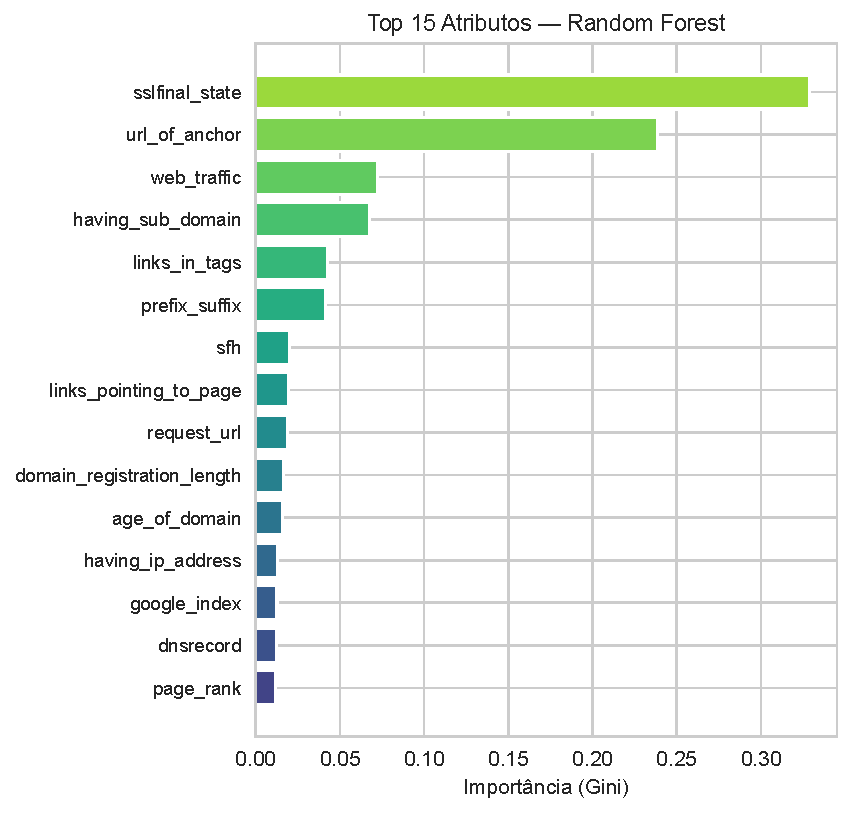
\includegraphics[width=\columnwidth]{importancia.pdf}
\caption{Importância (critério Gini) dos 15 atributos mais relevantes segundo
o \melhorModelo{}.}
\label{fig:importancia}
\end{figure}

\section{Conclusão}

Este trabalho comparou sete classificadores clássicos na tarefa de detecção
de phishing em URLs usando o dataset UCI Phishing Websites (\nTotal{} amostras,
\nFeatures{} atributos). \melhorModelo{} apresentou o melhor desempenho
($\text{F1} = \melhorFOne{}$, $\text{AUC-ROC} = \melhorAUC{}$), e o teste
de Friedman confirmou diferenças estatisticamente significativas entre os
modelos ($\chi^{2} = \friedmanChi{}$, $p \friedmanP{}$). A análise de
importância indicou que o estado do certificado SSL e a proporção de âncoras
externas são os atributos mais discriminativos. Como limitação, o dataset
utiliza atributos extraídos manualmente, o que implica latência adicional na
detecção em tempo real; trabalhos futuros poderiam investigar atributos léxicos
brutos da URL, dispensando o acesso ao conteúdo da página.

\bibliographystyle{sbc}
\bibliography{referencias}

\end{document}
